\newpage % Rozdziały zaczynamy od nowej strony.
\section{Opis teoretyczny rozwiązania}
W rozdziale przedstawione zostaną wszystkie założenia teoretyczne niezbędne do pełnego zrozumienia przedmiotu pracy i późniejszej interpretacji uzyskanych rezultatów. Na początku przedstawiona zostanie idea regulacji predykcyjnej wraz z algorytmem DMC oraz obiektem regulacji, który zostanie użyty w trakcie eksperymentów. W tej części pracy przydatne były opracowania \cite{stp2009} oraz \cite{tatjewski2016}. Następnie omówię architekturę sztucznej sieci neuronowej wraz z opisem funkcji aktywacji i metodą uczenia sieci. Tutaj szczególnie pomocne okazały się pozycje \cite{nielsen2015}, \cite{osowski2013} oraz \cite{wawrzynski2019}. Uwagę należy zwrócić tutaj na opis algorytmu OBD czyli użytą w tej pracy metodę upraszczania sieci neuronowej. Na końcu omówiona zostanie strategia, która została wykorzystana w trakcie wykonanych eksperymentów. Lektura rozdziału powinna zaznajomić czytelnika z wszystkimi kluczowymi zagadnieniami z punktu widzenia niniejszej pracy.

\subsection{Regulacja Predykcyjna}
Regulacja predykcyjna uznawana jest za jedną z zaawansowanych technik regulacji, które to zastąpiły uprzednio powszechnie stosowane regulatory PID. Dla wielowymiarowych i skomplikowanych procesów, regulacja w oparciu o identyfikacje jednego punktu charakterystyki obiektu, jak to wygląda w regulatorze PID, może okazać się nieefektywna. Rozwiązaniem jest tutaj wykorzystanie zasady przesuwanego horyzontu i wyznaczanie w każdej chwili \(kT\), gdzie T oznacza okres próbkowania, sekwencji przyszłych wartości sygnału sterującego. Idea każdego z algorytmów regulacji predykcyjnej polega na wyznaczeniu w każdej iteracji wektora przyrostów sygnału sterującego.
\begin{equation}
\Delta U(k) \, = \, [\Delta u(k|k)\quad \Delta u(k+1|k)\quad \Delta u(k+2|k)\quad ... \quad \Delta u(k + N_u - 1|k)]^T
\end{equation}
gdzie przez \(N_u\) oznaczamy horyzont sterowania, a notacja \(\Delta u(k+p|k)\) oznacza przyrost sygnału sterującego obliczony w chwili \(k\), który ma być wykorzystany do sterowania w chwili \(k+p\). W istocie jednak do sterowania wykorzystuje się tylko pierwszą wartość wyznaczanego wektora i prawo regulacji w kolejnych iteracjach przyjmuje postać
\begin{equation}
u(k) \, = \, u(k|k) \, = \, \Delta u(k|k) + u(k-1)
\end{equation}

\subsubsection{Algorytm DMC}
Główna idea algorytmu DMC (Dynamic Matrix Control), przedstawionego w \cite{dmc1979}, opiera się na wykorzystaniu modelu odpowiedzi skokowej do predykcji. Algorytm DMC identyfikuje dynamikę obiektu regulacji za pomocą dyskretnych odpowiedzi skokowych, które są reakcją wyjścia w kolejnych okresach próbkowania na jednostkowy skok sygnału sterującego. Na rysunku 3.1. przedstawiono przykładową odpowiedź skokową obiektu regulacji, który to opisany zostanie w kolejnym podrozdziale. Następnie tak wyznaczona odpowiedzi skokowa obiektu \(\{s_1,\, s_2,\, s_3,\, ...\, s_D \}\) wykorzystywana jest w algorytmie DMC do wyznaczenia najbardziej optymalnych wartości sterowania. Wielkość \(D\) oznacza horyzont dynamiki obiektu i powinna zostać dobrana eksperymentalnie do takiej wartości po której wyjście obiektu ulega stabilizacji. 
\begin{figure}[!h]
    \label{fig:Odpowiedz-skokowa}
    \centering 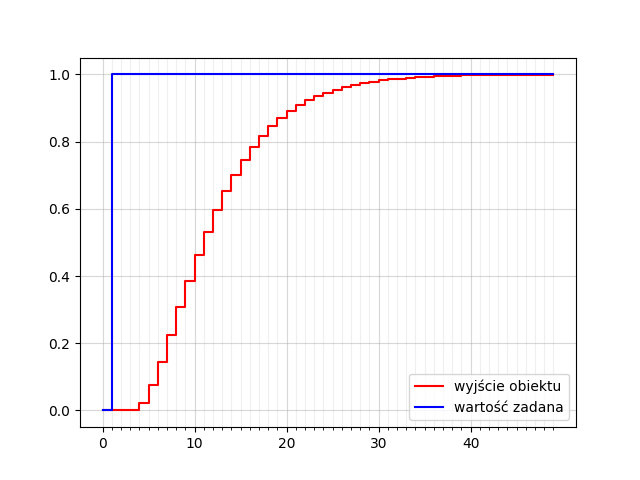
\includegraphics[width=0.7\linewidth]{Odpowiedz_skokowa.png}
    \caption{Przykładowa odpowiedź wyjścia obiektu na jednostkowy skok sterowania}
\end{figure}
\par W każdej iteracji wektor (1) wyznaczany jest w wyniku minimalizacji wskaźnika jakości, który zapisany w formie wektorowo-macierzowej przyjmuje postać
\begin{equation}
J(k) \, = \, \left\| Y^{zad}(k) - \hat{Y}(k) \right\|_{\bm{\Psi}}^2 \,+ \,\left\| \Delta U(k) \right\|_{\bm{\Lambda}}^2
\end{equation}
gdzie wektory wartości zadanej \( Y^{zad}(k) \) oraz prognozowanej trajektorii wyjścia \( \hat{Y}(k) \) o długości \( N \) będącej horyzontem predykcji definiowane są w następujący sposób
\begin{equation}
Y^{zad}(k) =
	 \begin{bmatrix}
		y^{zad}(k+1|k) \\
		\vdots \\
		y^{zad}(k+N|k)
	\end{bmatrix} , \quad
\hat{Y}(k) = 
	\begin{bmatrix}
		\hat{y}(k+1|k) \\
		\vdots \\
		\hat{y}(k+N|k)
	\end{bmatrix}
\end{equation}
macierze \( \Lambda\) oraz \( \Psi\) są macierzami diagonalnymi, a w większości przypadków przyjmują postać macierzy identyczności i takie również założenie przyjęte zostało w tej pracy. 
\par Następnie korzystając z przekształceń szczegółowo omówionych w \cite{stp2009} zapisujemy funkcję kryterialną w postaci
\begin{equation}
J(k) \, = \, \left\| Y^{zad}(k) - Y(k) - \bm{M}^P \Delta U^P(k) - \bm{M} \Delta U(k) \right\|_{\bm{\Psi}}^2 \,+ \,
\left\| \Delta U(k) \right\|_{\bm{\Lambda}}^2
\end{equation}
gdzie macierz \(M \) o wymiarowości \( N \times N_u \) ma strukturę
\begin{equation}
\bm{M} = 
	\begin{bmatrix}
		s_1 & 0 & \cdots & 0 \\
		s_2 & s_1 & \cdots & 0 \\
		\vdots & \vdots & \ddots & \vdots \\
		s_N & s_{N-1} & \cdots & s_{N-N_u+1}
	\end{bmatrix}
\end{equation}, 
macierz \(M^P \) o wymiarowości \( N \times (D-1) \) 
\begin{equation}
\bm{M^P} = 
	\begin{bmatrix}
		s_2 - s_1 & s_3 - s_2 & \cdots & s_D - s_{D-1} \\
		s_3 - s_1 & s_4 - s_2 & \cdots & s_{D+1} - S_{D-1}  \\
		\vdots & \vdots & \ddots & \vdots \\
		s_{N+1} - s_1 & s_{N+2} - s_2 & \cdots & s_{N+D-1} - s_{D-1}
	\end{bmatrix}
\end{equation}, 
natomiast wektor \( \Delta U^P(k) \) zawiera przeszłe \(D-1\) wartości zamian sygnału sterującego \(\Delta u(k-i)\). 

\par Zauważając, że funkcja jest ściśle wypukła, przyrównujemy do zera wektor gradientu funkcji i otrzymujemy wektor optymalnych przyrostów sterowania
\begin{equation}
\Delta U(k) \, = \, (\bm{M}^T\bm{\Psi}\bm{M}+\bm{\Lambda})^{-1}\bm{M}^T\bm{\Psi}(Y^{zad}(k) - Y(k) - \bm{M}^P \Delta U^P(k))
\end{equation}, 
gdzie początkową część możemy zapisać w formie 
\begin{equation}
\bm{K} \, = \, (\bm{M}^T\bm{\Psi}\bm{M}+\bm{\Lambda})^{-1}\bm{M}^T\bm{\Psi}
\end{equation}
gdzie macierz \( \bm{K}\) o wymiarowości \( N_u \times N \) wyznacza jest jednokrotnie w trakcie projektowania algorytmu. Równanie (8) stanowi podstawą działania algorytmu i posłuży do dalszej bezpośredniej implementacji.

\subsubsection{Obiekt regulacji}
Aby przeprowadzić niezbędne eksperymenty i dokonać porównania różnych regulatorów niezbędne jest wybranie i zaimplementowanie obiektu regulacji. W niniejszej pracy w roli obiektu wykorzystany zostanie człon inercyjny drugiego rzędu z opóźnieniem. Wybrany układ najłatwiej przedstawić w postaci równania różnicowego 
\begin{equation}
y(k) \, = \, b_1u(k-T_d-1) + b_2u(k-T_d-2)-a_1y(k-1)-a_2y(k-2)
\end{equation}
gdzie 
\begin{align*}
a_1 \, &= \, -\alpha_1 -\alpha_2 \\
a_2 \, &= \, \alpha_1\alpha_2 \\
\alpha_1 \, &= \, e^{-\frac{1}{T_1}} \\
\alpha_2 \, &= \, e^{-\frac{1}{T_2}} \\
b_1 \, &= \, \frac{K}{T_1 - T_2}[T_1(1-\alpha_1)-T_2(1-\alpha_2)] \\
b_2 \, &= \, \frac{K}{T_1 - T_2}[\alpha_1 T_2(1-\alpha_2)-\alpha_2 T_1(1-\alpha_1)]
\end{align*}

\par Dzięki takiej prezentacji i implementacji ogólnej klasy układu regulacji mamy możliwość identyfikacji poszczególnych układów poprzez cztery parametry \( T_1, \, T_2, \, K, \, T_d \). Jest to istotna własność dzięki, której w łatwy sposób można dokonywać modyfikacji obiektu i sprawdzać zachowanie regulatora w poszczególnych przypadkach.

\par Dla lepszego zrozumienia zagadnienia warto przyjrzeć się przebiegowi regulacji predykcyjnej DMC dla jednego wybranego układu regulacji. Eksperyment przedstawiony na rysunku 3.2 przeprowadzony został dla następujących parametrów \( T_1=5, \, T_2=4, \, K=1, \, T_d=3 \). Warto zaznaczyć, że dla tego samego układ wcześniej pokazana została odpowiedź skokowa z rysunku 3.1.  
\begin{figure}[!h]
    \label{fig:Regulacja-DMC}
    \centering 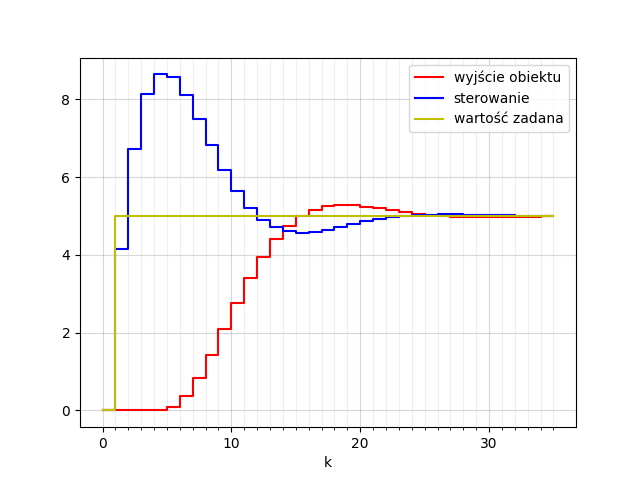
\includegraphics[width=0.7\linewidth]{Regulacja_DMC.png}
    \caption{Regulacja DMC dla wybranego obiektu}
\end{figure}

\subsection{Sztuczne Sieci Neuronowe}
Sztuczne sieci neuronowe stanowią jedną z najczęściej omawianych metod przetwarzania informacji w ostatnich lat. Wielką popularność zyskały niewątpliwie dzięki swojemu interdyscyplinarnemu charakterowy, łącza one osiągnięcia biocybernetyki, elektroniki, matematyki stosowanej, statystyki oraz automatyki. Istotą działania sieci neuronowych jest próba odtworzenia zjawisk zachodzących w systemach nerwowych istot żywych poprzez zastosowanie nowoczesnych rozwiązań technologicznych.

\subsubsection{Architektura sieci}
Bazując na literaturze omówionej w poprzednim rozdziale w niniejszej pracy wykorzystana zostanie jednokierunkowa sieć typu sigmoidalnego o jednej warstwie ukrytej. Jest to jedna z najprostszych możliwych struktur, w której występują trzy warstwy neuronów wejściowa, ukryta i wyjściowa. Liczba neuronów w warstwie wejściowej i wyjściowej ściśle zależy od wymiarowości danych, natomiast największy wpływ na efektywność działania sieci ma właściwy dobór liczby neuronów w warstwie ukrytej. Poglądowy schemat jednokierunkowej sieci neuronowej przedstawiony został na rysunku 3.3. Na schemacie pokazano dwie warstwy ukryte dla lepszego zrozumienia połączeń między kolejnymi warstwami. W wyjściowej strukturze pojedynczy neuron danej warstwy połączony jest ze wszystkimi neuronami kolejnej warstwy. Liczba połączeń może być później redukowana z wykorzystywaniem algorytmu OBD, który opisany zostanie w dalszej części. 
%struktura sieci
\begin{figure}[!h]
    \label{fig:struktura-sieci}
    \centering 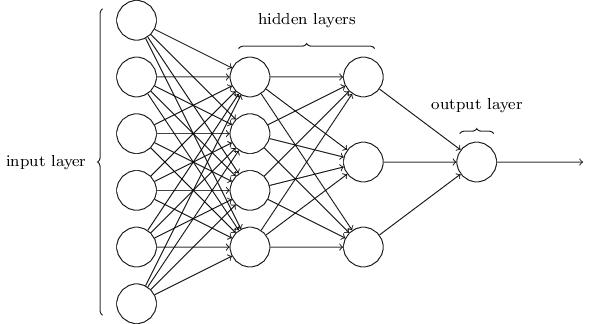
\includegraphics[width=0.7\linewidth]{struktura_sieci1.png}
    \caption{Schemat poglądowy struktury sieci. Źródło: \cite{nielsen2015} }
\end{figure}

\par Kluczowym dla zrozumienia działania całej sieci neuronowej jest przekształcenie zachodzące w obrębie pojedynczego neuronu. Model neuronu przedstawiony został na rysunku 3.4. Wejścia do danego neuronu zostają przemnożone przez odpowiednie wagi, a następnie zsumowane. Następnie obliczoną sumę wykorzystujemy jako argument funkcji aktywacji przez co otrzymujemy wyjście z danego neuronu. Jedną z najczęściej stosowanych funkcji aktywacji jest funkcja sigmoidalna unipolarna o postaci 
\begin{equation}
f(z) \, = \, \frac{1}{1+e^{-z}}, 
\end{equation}
której przebieg widzimy na rysunku 3.5. Warto zauważyć, że w obrębie dostatecznie małych i dużych wartości wejścia do funkcji sigmoidalnej następuje jej stabilizacja, a co za tym idzie tak zwana stabilizacja całego neuronu.
%model neuronu
\begin{figure}[!h]
    \label{fig:struktura-sieci}
    \centering 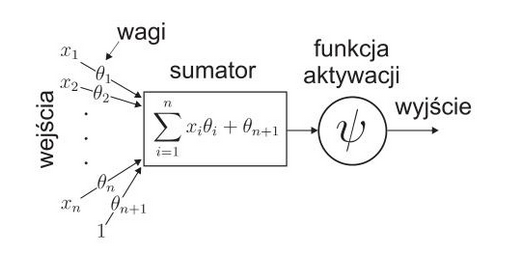
\includegraphics[width=0.6\linewidth]{model_neuronu.png}
    \caption{Model neuronu. Źródło: \cite{wawrzynski2019} }
\end{figure}
%funkcja aktywacji
\begin{figure}[!h]
    \label{fig:sigmoid}
    \centering 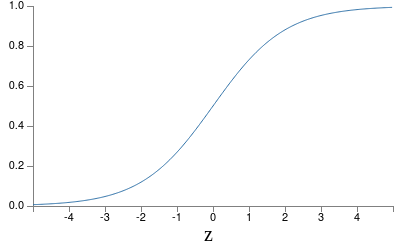
\includegraphics[width=0.5\linewidth]{sigmoid.png}
    \caption{Przebieg funkcji sigmoidalnej unipolarnej. Źródło: \cite{nielsen2015}}
\end{figure}

\subsubsection{Wsteczna propagacja gradientu}
Uczenie sieci neuronowej możemy opisać w postaci następującego problemu. Mamy dany zbiór przykładów uczących postaci \(<x,y^d> \), wektor wyjść sieci \(\bar{f}(x;\theta)\) oraz pewną funkcje straty mierzącą rozbieżność między \(y^d \) a wektorem wyjść obliczonym przez sieć, która w naszym przypadku przyjmuje postać funkcji kwadratowej, 
\begin{equation}
q(\bar{f}(x;\theta)) \, = \, \left\| \bar{f}(x;\theta) - y^d \right\|^2. 
\end{equation}
Zadaniem algorytmu uczenia jest tak dobrać wartości parametrów \( \theta \) czyli kolejnych wag sieci, aby osiągnąć minimum funkcji straty co z kolei opiera się na wyznaczeniu gradientu funkcji kosztu po danych parametrach, czyli wektora
\begin{equation}
\frac{dq(\bar{f}(x;\theta))}{d\theta^T}. 
\end{equation}
W praktyce wyprowadzenie konkretnych formuł na gradient funkcji za pomocą funkcji wejścia i wag może być zbyt skomplikowane. Aby uniknąć tej niedogodności stosuje się metodę wstecznej propagacji. Celem tej metody jest obliczenie pochodnych cząstkowych \( \frac{\partial q}{\partial w_{jk}^l} \) oraz \( \frac{\partial q}{\partial b_j^l} \), gdzie \( w_{jk}^l \) oznaczą wagę łączącą k-ty neuron warstwy l-1 z j-tym neuronem warstwy l, natomiast \(b_{j}^l\) oznacza wyraz wolny j-tego neuronu warstwy l. Dla łatwiejszej prezentacji algorytmu wprowadzamy wartość \( \delta_j^l \, = \, \frac{\partial q}{\partial z_j^l} \), którą możemy interpretować jako błąd j-tego neuronu l-tej warstwy czyli pochodną cząstkową po wartości zwracanej przez sumator z rysunku 3.4. 

\par Teraz możemy przedstawić algorytm wstecznej propagacji za pomocą czterech równań. Pierwszym z nich jest wyrażenie na wartości \(\delta_j^l \) dla warstwy wyjściowej \( L \) o postaci 
\begin{equation}
\delta_j^L \, = \, \frac{\partial q}{\partial a_j^L}f^{\prime}(z_j^L),
\end{equation}
które dla kwadratowej funkcji kosztu w wersji macierzowej zapisujemy jako
\begin{equation}
\delta_j^L \, = \, (a^L - y^d)\odot f^{\prime}(z_j^L),
\end{equation}
gdzie symbol \( \odot \) oznacza iloczyn Hadamarda, \( f \) jest zdefiniowaną wcześniej funkcją aktywacji, natomiast \( a_j^L = f(z_j^l) \). 
Drugim równaniem jest wyrażenie błędów neuronów l-tej warstwy poprzez wartości błędów l+1-tej warstwy. Zapis macierzowy wygląda następująco 
\begin{equation}
\delta^l \, = \, ((w^{l+1})^T\delta^{l+1}) \odot f^{\prime}(z^l). 
\end{equation}
Za pomocą równań (15) i (16) możemy wyznaczyć wektory \( \delta_j^l \) dla każdej z warstw. Dwa kolejne równania opisują powiązanie kolejnych pochodnych cząstkowych funkcji kosztu z wyznaczonymi za pomocą dwóch pierwszych równań wektorami. Kolejno dla wyrazów wolnych
\begin{equation}
\frac{\partial q}{\partial b_j^l} \, = \, \delta_j^l , 
\end{equation}
oraz wag przypisanych do poszczególnych połączeń
\begin{equation}
\frac{\partial q}{\partial w_{jk}^l} \, = \, a_k^{l-1}\delta _j^l
\end{equation}
\par Równanie 15 - 18 stanowią bezpośrednią podstawę do póżniejszej implementacji. Wyprowadzenie tych równań zostało pominięte w pracy, z uwagi że algorytm wstecznej propagacji nie jest głównym aspektem niniejszej pracy, jednak uważny czytelnik może znaleźć pełny opis w pozycjach \cite{osowski2013} oraz \cite{nielsen2015}. 

\subsubsection{Algorytm OBD}
Dzięki opisanej wcześniej metodzie uczenia sieci neuronowej mamy możliwość minimalizacji błędu popełnianego przez sieć na danych uczących i weryfikujących. Niestety nie daje to pewności, że ostateczny dobór parametrów jest optymalny ze względu na wrażliwość trenowanej sieci na początkowy dobór parametrów uczenia oraz poszczególnych wartości wag. Zgodnie z \cite{osowski2013} rozwiązaniem może być tutaj zastosowanie metod redukcji sieci, a za jedną z lepszych możemy uznać algorytm OBD (Optimal Brain Damage) zaproponowany przez LeCun \cite{lecun1989}. Wskazany algorytm należy do klasy wrażliwościowych metod redukcji sieci i jego podstawowym zadaniem jest zmniejszenie liczby powiązań między-neuronowych a co za tym idzie uproszczenie struktury sieci. 
\par Idea algorytmu OBD polega na przypisaniu każdej z wag miary, która określi wrażliwość sieci na zmianę tej konkretnej wagi. Następnie wagi o najmniejszej wrażliwości mogą zostać usunięte co nie powinno wpłynąć w istotny sposób na działanie sieci, a za to pozwolić na uproszczenie jej struktury. Twórca algorytmu za miarę ważności danej wagi proponuje współczynnik asymetrii (ang. saliency), który zdefiniowany zostaje w następujący sposób
\begin{equation}
S_i \, = \, \frac{1}{2} \frac{\partial^2q}{\partial \theta_i^2} * \theta_i^2 .
\end{equation} 
Podstawą do zdefiniowania miary było rozwinięcie funkcji celu \(q\) w szereg Taylora i na tej podstawie znalezienie parametrów, których usunięcie będzie miało najmniejszy wpływ na  \(q\). Wyznaczenie pełnej macierzy Hessego \(H\) w większości przypadków staje się niemożliwie ze względu na złożoność obliczeniową. Z tego powodu LeCun wykorzystał fakt, że wobec dodatniej określoności hesjanu macierz \(H\) jest diagonalnie dominująca. Zasadnym jest zatem uwzględnienie jedynie składników diagonalnych \( h_{ii} \), które to możemy wyznaczyć dostosowując metodę wstecznej propagacji poprzednio omówioną dla pierwszych pochodnych. 
\par Podtrzymując założenie o kwadratowej funkcji kosztu dla każdego przykładu uczącego wyliczamy miarę
\begin{equation}
h_{ii} \, = \, \frac{\partial^2q}{\partial (w_{jk}^l)^2}, 
\end{equation}  
gdzie \( w_{jk}^l \) jest połączeniem pomiędzy neuronami zdefiniowanym przy prezentacji algorytmu wstecznej propagacji.
Formułę możemy rozwinąć do postaci 
\begin{equation}
\frac{\partial^2 q}{\partial (w_{jk}^l)^2} \, = \, \frac{\partial^2 q}{\partial (z_j^{l})^2}(a_k^{l-1})^2 , 
\end{equation}
i zastosować wsteczną propagację w postaci
\begin{equation}
\frac{\partial^2q}{\partial (z_k^{l})^2} \, = \, f^{\prime}(z_k^l)^2 \sum_j (w_{jk}^{l+1})^2 \frac{\partial^2 q}{\partial (z_j^{l+1})^2} + f^{\prime \prime}(z_k^l) \frac{\partial q}{\partial a_k^l}. 
\end{equation}
Dodatkowo poprzez zastosowanie aproksymacji Levenberga-Marquardta możemy uprościć wzór do postaci
\begin{equation}
\frac{\partial^2q}{\partial (z_k^{l})^2} \, = \, f^{\prime}(z_k^l)^2 \sum_j (w_{jk}^{l+1})^2 \frac{\partial^2 q}{\partial (z_j^{l+1})^2}
\end{equation}
co dodatkowo daje gwarancję, że wyznaczane aproksymacje drugich pochodnych nie będą ujemne.
Przed zastosowaniem powyższego wzoru niezbędne jest wyznaczenie wartości początkowej czyli drugich pochodnych dla ostatniej warstwy sieci neuronowej. Ponownie stosując wspomnianą wcześniej aproksymację otrzymujemy wzór postaci
\begin{equation}
\frac{\partial^2q}{\partial (z_k^{L})^2} \, = \, 2f^{\prime}(z_k^{L})^2. 
\end{equation}
\par Po wyznaczeniu wartości diagonalnych \( h_{ii} \) należy uśrednić je po wszystkich przykładach uczących i na tej podstawie według wzoru (19) wyznaczyć współczynniki asymetrii, zgodnie z którymi przycinane będą kolejne wagi sieci. Ogólną procedurę algorytmu OBD zapisać możemy w następujących krokach: 
\begin{enumerate}
 \item Wybór właściwej architektury sieci
 \item Pełne wytrenowanie danej struktury przy użyciu jednej z metod uczenia, na przykład wstecznej propagacji
 \item Obliczenie wartości diagonalnych macierzy Hessego czyli współczynników \( h_{ii} \) 
 \item Wyznaczenie współczynników asymetrii \( S_i \)
 \item Posortowanie parametrów rosnąco według współczynników \( S_i \)
 \item Usunięcie najmniej znaczących wag
 \item Powtórzenie procedury od punktu 2, aż do osiągnięcia pożądanego kryterium wyjścia  na danych weryfikujących
\end{enumerate}
Warto zauważyć, że usunięcie wagi odbywa się poprzez ustawienie jej wartości na zero i przypisanie odpowiedniej maski, która uniemożliwia metodzie wstecznej propagacji ponowną modyfikację parametru.  

\subsection{Strategia eksperymentów}
Opisane założenia teoretyczne stanowią podstawę do implementacji rozwiązania i przeprowadzenia eksperymentów praktycznych, których wyniki przedstawione zostaną w kolejnym rozdziale. Przed przystąpieniem do prezentacji wyników warto jednak jeszcze opisać schemat według, którego zostaną one przeprowadzone. Pozwoli to czytelnikowi na ewentualną samodzielną interpretację wyników i będzie prowadziło do lepszego zrozumienia wniosków płynących z pracy. Poniższy schemat stanowi jedynie zwięzły opis strategi, a wszystkie szczegóły wskazane zostaną we właściwym rozdziale. 
\par Pierwszym etap jest wygenerowanie danych, które następnie stanowić będą przykłady uczące i weryfikujące zarówno dla algorytmu wstecznej propagacji jak i OBD. Generacja danych polega na przeprowadzeniu symulacji z wykorzystaniem regulatora DMC i zdefiniowanego obiektu regulacji. Warto zwrócić uwagę na fakt, że dane uczące i weryfikujące generowane będą oddzielnie, dzięki czemu działanie sieci neuronowej weryfikowane będzie z wykorzystaniem przykładów symulacji niewystępujących w danych uczących. Jednak przed zastosowaniem otrzymanych danych w procedurze uczenia sieci niezbędne jest ich przeskalowanie do wartości z zakresu od -1 do 1. Jest to niezbędny krok wymuszony przez rodzaj zastosowanej funkcji aktywacji. Wartym zauważenia jest fakt, że koniecznym było zastosowanie modułu skalującego pozwalającego na transformację danych wejściowych w dwie strony. Sieć neuronowa wykorzystana zostanie jako regulator, a zatem procedura odwrotnego skalowania jest tutaj niezbędna. 
\par Następnie należy wytrenować sieć neuronową z wykorzystaniem opisanej metody wstecznej propagacji. Z uwagi na fakt, że kolejnym krokiem będzie wykorzystanie algorytmu OBD do redukcji sieci, należy zastosować lekko zmodyfikowaną strategię względem klasycznego podejścia do uczenia sieci neuronowej. Algorytm OBD wymaga aby funkcja celu była w swoim minimum, a zatem konieczne jest pełne wytrenowanie sieci na danych uczących bez stosowania kryterium wyjścia na danych weryfikujących. Algorytm uczenia sieci zakończy swoje działanie gdy zmiany funkcji kosztu w kolejnych iteracjach będą dostatecznie małe. Eksperymenty powtórzone zostaną dla różnej ilości neuronów w warstwie ukrytej oraz różnych wartości współczynnika uczącego sieci. Pozwoli to na wybór najbardziej optymalnej architektury przed przystąpieniem do procedury redukcji sieci. 
\par Kolejno zastosujemy procedurę OBD dla optymalnej struktury sieci. Redukcja sieci zgodnie z opisaną wcześniej procedurą będzie kontynuowana aż zmiana funkcji kosztu na danych weryfikujących osiągnie dostatecznie mała wartość. Dzięki takiemu podejściu otrzymamy sieć neuronową, która powinna posiadać wysokie zdolności generalizacji postawionego przed nią zadania. W celu weryfikacji otrzymanego rezultatu przeprowadzona zostanie symulacja danego układu regulacji dla różnych wartości zadanych z wykorzystaniem sieci neuronowej oraz regulatora DMC. W obu przypadkach wyznaczony zostanie błąd średnio-kwadratowy i na tej podstawie możliwe będzie porównanie dwóch zastosowanych metod i weryfikacja czy sieć neuronowa jest w stanie zastąpić klasyczny regulator.
\par Ostatnim etapem prowadzonych badań będzie przetestowanie działania sieci neuronowej jako regulatora zmodyfikowanych obiektów regulacji. Wykorzystana zostanie tutaj wcześniej opisana własność łatwej zmiany obiektu regulacji poprzez dobór odpowiednich parametrów. Przeanalizowane zostanie również działanie sieci dla bardziej skomplikowanych przebiegów regulacji, przykładowo wielokrotnego skoku wartości zadanej.
\vspace{10mm}
\par W rozdziale przedstawione zostały wszystkie niezbędne opisy i założenia teoretyczne pozwalające na pełne zrozumienie omawianego zagadnienia. Zaprezentowane wzory i struktury stanowią bezpośrednią podstawę do praktycznej implementacji rozwiązanie, której najważniejsze części przedstawione zostaną w kolejnym rozdziale. Dodatkowo lektura tego rozdziału powinna umożliwić czytelnikowi samodzielną interpretację wyników i dokładniejsze zrozumienie charakteru pracy.   
      


